% Architecture pipeline figure for pytscope's README ("How it works").
%
% Build (from this directory):
%   pdflatex -interaction=nonstopmode architecture.tex
%   convert -density 300 architecture.pdf -trim +repage -background white \
%           -alpha remove -alpha off architecture.png
%
% A pre-rendered PNG (architecture.png) is committed alongside this source so
% the README can embed it directly without requiring readers to build LaTeX.
\documentclass{article}
\usepackage[margin=0pt, paperwidth=20cm, paperheight=24cm]{geometry}
\usepackage{tikz}
\usetikzlibrary{arrows.meta, positioning, fit, backgrounds}
\pagestyle{empty}

% Explicit RGB colors — the amber/teal/violet "hardware panel" palette,
% defined directly so the figure doesn't depend on optional xcolor name sets.
\definecolor{psAmber}{RGB}{217,144,29}
\definecolor{psTeal}{RGB}{27,138,143}
\definecolor{psViolet}{RGB}{121,75,160}
\definecolor{psRed}{RGB}{196,57,57}

\begin{document}
\noindent
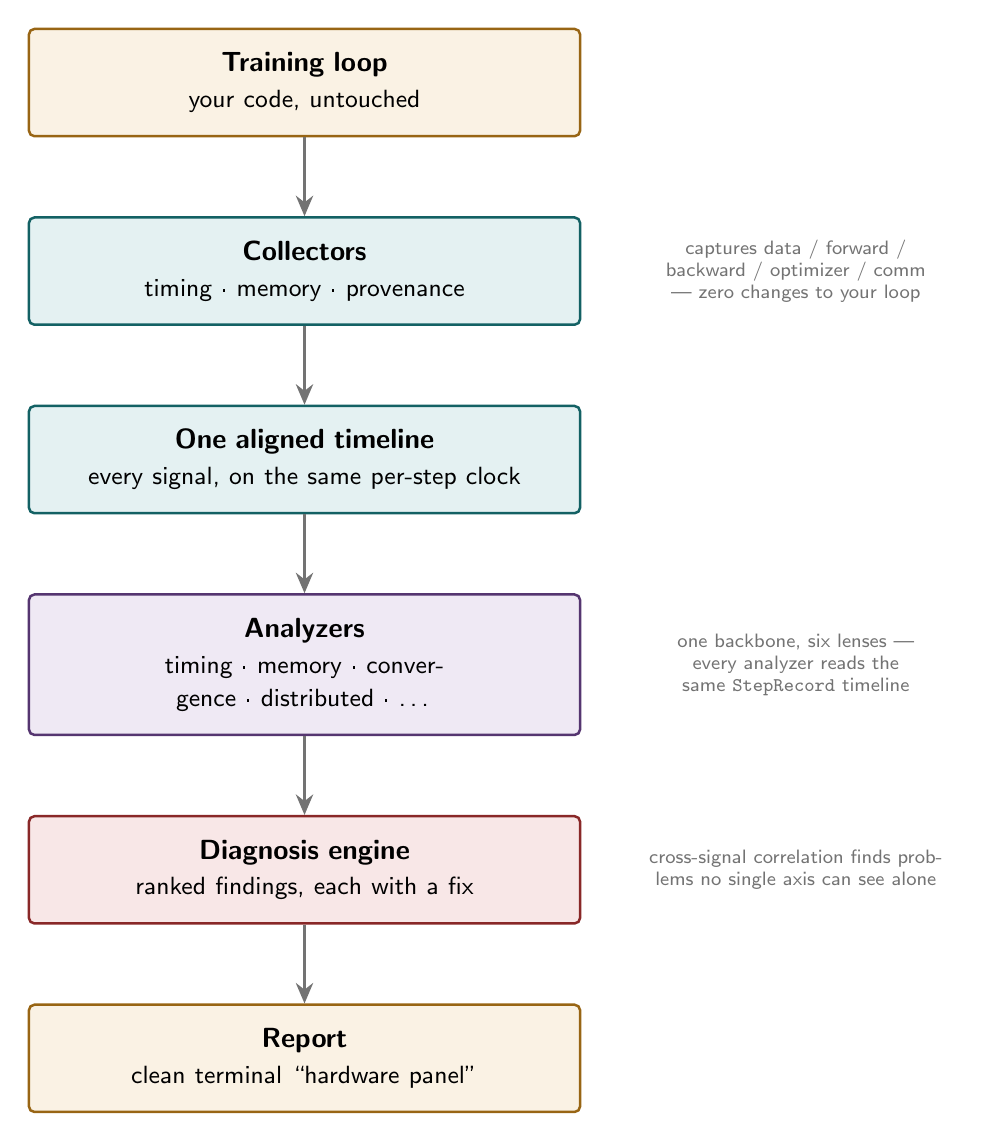
\begin{tikzpicture}[
  font=\sffamily,
  node distance=10mm and 10mm,
  stage/.style={
    rectangle, rounded corners=2pt, draw=#1!70!black, fill=#1!12,
    text width=64mm, align=center, minimum height=13mm,
    inner sep=3mm, line width=0.9pt
  },
  caption/.style={font=\sffamily\scriptsize, text=black!55, align=center},
  flow/.style={-{Stealth[length=2.6mm, width=2.2mm]}, line width=1pt, draw=black!55},
]

% --- Pipeline stages, top to bottom ---------------------------------------
\node[stage=psAmber]                                 (loop)  {\textbf{Training loop}\\[1pt] \small your code, untouched};
\node[stage=psTeal,    below=of loop]                (coll)  {\textbf{Collectors}\\[1pt] \small timing · memory · provenance};
\node[stage=psTeal,    below=of coll]                (line)  {\textbf{One aligned timeline}\\[1pt] \small every signal, on the same per-step clock};
\node[stage=psViolet,  below=of line]                (an)    {\textbf{Analyzers}\\[1pt] \small timing · memory · convergence · distributed · \ldots};
\node[stage=psRed,     below=of an]                  (diag)  {\textbf{Diagnosis engine}\\[1pt] \small ranked findings, each with a fix};
\node[stage=psAmber,   below=of diag]                (rep)   {\textbf{Report}\\[1pt] \small clean terminal ``hardware panel''};

% --- Arrows ----------------------------------------------------------------
\foreach \a/\b in {loop/coll, coll/line, line/an, an/diag, diag/rep}
  \draw[flow] (\a) -- (\b);

% --- Side annotations -------------------------------------------------------
\node[caption, right=7mm of coll, text width=38mm]  {captures data / forward / backward / optimizer / comm — zero changes to your loop};
\node[caption, right=7mm of an,   text width=38mm]  {one backbone, six lenses — every analyzer reads the same \texttt{StepRecord} timeline};
\node[caption, right=7mm of diag, text width=38mm]  {cross-signal correlation finds problems no single axis can see alone};

\end{tikzpicture}
\end{document}
